\documentclass[a4paper,14px]{article}
\usepackage[left=2cm,right=2cm,top=2cm,bottom=2cm]{geometry}
\usepackage{graphicx}
\usepackage{float}

\title{``SITIO WEB PARA LA GESTIÓN Y PROMOCIÓN DE CONGRESOS INTERNACIONALES EN INSTITUCIONES DE EDUCACIÓN SUPERIOR''}

\author{Equipo de desarrollo \\ Ing. Stalin Francis Quinde (Team Developer) \\ Ing. Joseph Cruel (Product Owner) \\ Ing Xavier Garcia Cervantes. (Team Developer }
\begin{document}
\maketitle

\section{Antecedente}
\label{sec:antecedente}
La Facultad de Ingenierías de la Universidad Técnica Luis Vargas Torres (UTLVTE), organizó un congreso internacional llamado \textbf{``MIRADAS Y TENDENCIAS  DE LAS CIENCIAS INGENIERILES (MTCI) UTLVTE-2022''}, para lo cual necesitaba una plataforma web que le permitiera gestionar y difundir la información que  fue generada desde el momento de su concepción, hasta la culminación que se da con la presentación de las ponencias nacionales e internacionales.\\

Para lograr este objetivo tres docentes de la Facultad se apoyo en la carrera de Tecnología de la Información de la UTLVTE, donde docentes con experiencia en desarrollo web evaluaron varias alternativas a fin de poder aplicar la mejor solución en función de las necesidad y limitaciones que se presentaron en el levantamiento de la información.\\

De todas las soluciones ya existentes, ninguna se ajustaba de forma precisa a las restricciones de este evento, las cuales eran  gran variedad de recursos multimedia, facilidad para navegar desde dispositivos móviles y  más que todo bajo presupuesto para su desarrollo, ya que por ser un evento sin fines de lucro pero de gran nivel académico; existian alternativas comerciales que resultaron complejas de aprender y con muchas limitación en su versión libre; otras, muy buenas por cierto, resultaban costosas para poder ser utilizadas.\\

Se decidió que al contar con docentes con conocimientos y experiencias en el desarrollo web,  se podía crear un  sitio web propio, para poder  cumplir con el propósito a pesar de las restricciones antes indicadas.\\

Así nace el  ``Sitio Web para la gestión y promoción de congresos internacionales en instituciones de educación superior'' desarrollado por docentes de la UTLTE , el cual se constituye en un  conjunto de programas que utilizan las  herramientas,  html,css,javascrip, php, y mysql; y que se alojan al lado del Servidor Web para poder guardar, recuperar y mostrar la información multimedia de una forma sencilla, sistemática y ordenada desde y en cualquier parte del mundo a través de internet.\\

\section{Descripción de la arquitectura resumida}
\label{sec:descripcion-de-la}


En la gráfica siguiente se muestra de forma resumida como funciona el sitio, los programas estarán alojados en un servidor web (o web server) donde se contrato un hosting que se accede con el  dominio ``congresoutlvte.org'' el cual se comunica vía protocolo \textbf{http} con programas navegadores que se encuentran instalados en máquina situadas en cualquier parte del mundo, desde donde el usuario puede solicitar(request) información  que ha sido guardada. \\


\begin{figure}[H]
  \centering
  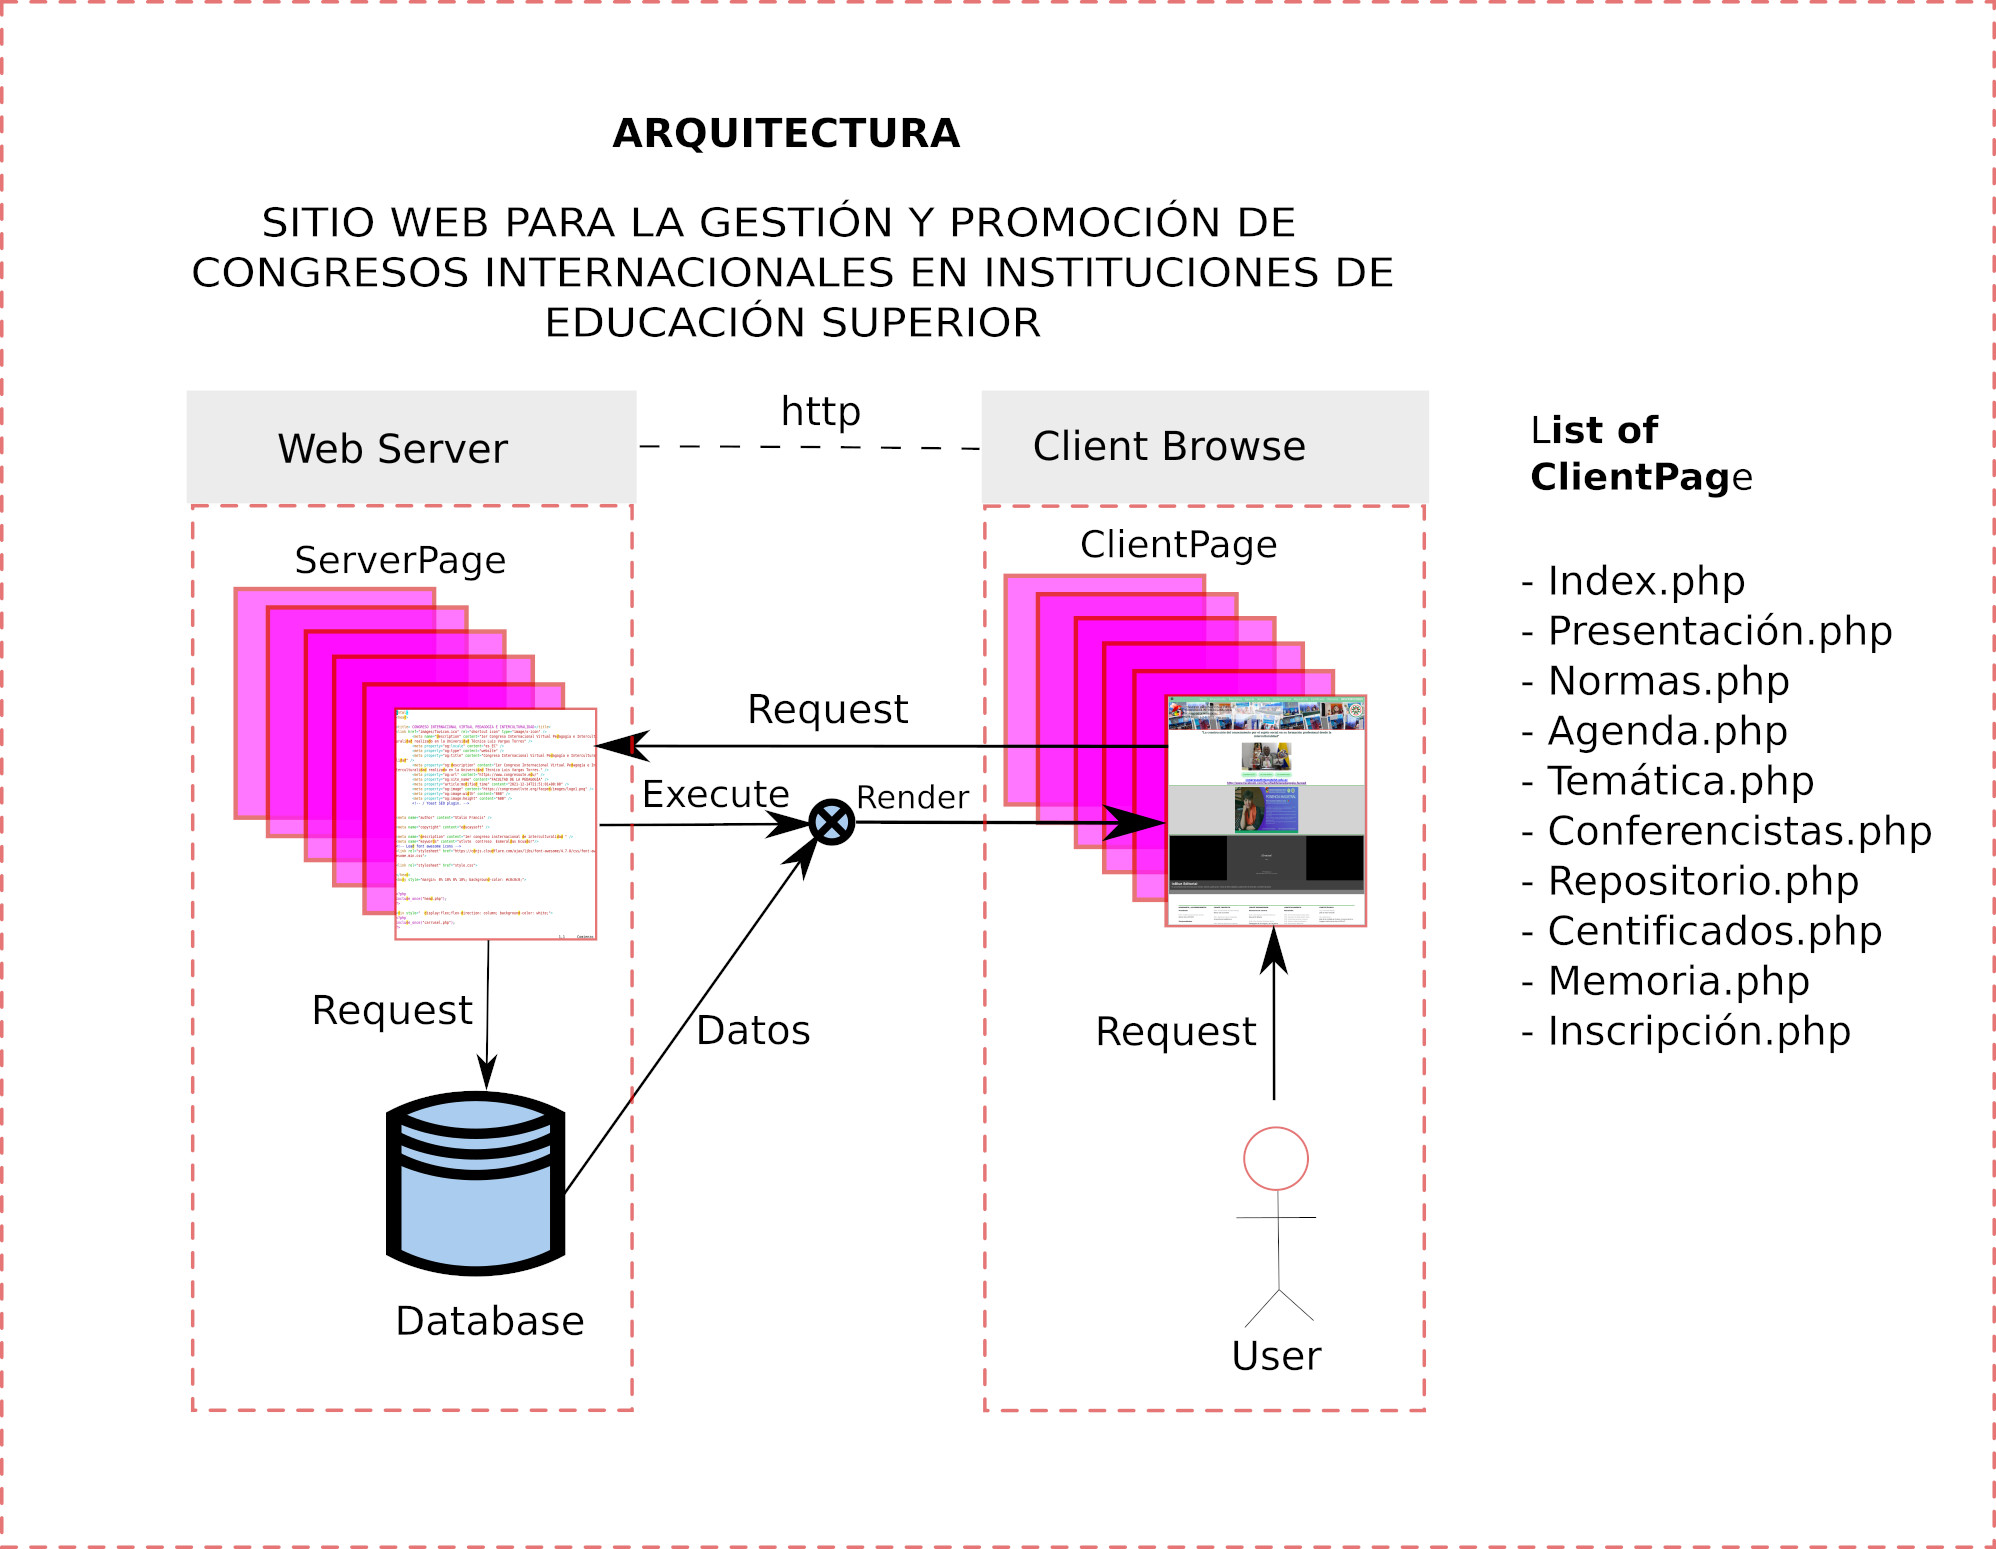
\includegraphics[scale=0.3]{congresoweb.jpg}
  \caption{Arquitectura resumida}
  \label{fig:arquitectura}
\end{figure}


\newpage
\subsection{Página principal}
\label{sec:pagina-principal}

En la figura 2 se muestra parte de la página principal del sitio web donde se pone a disposición información como logo de la universidad, banner promocional del congreso, resumen del congreso y fecha destacadas.

\begin{minipage}[H]{0.45\linewidth}
\begin{figure}[H]
  \centering
  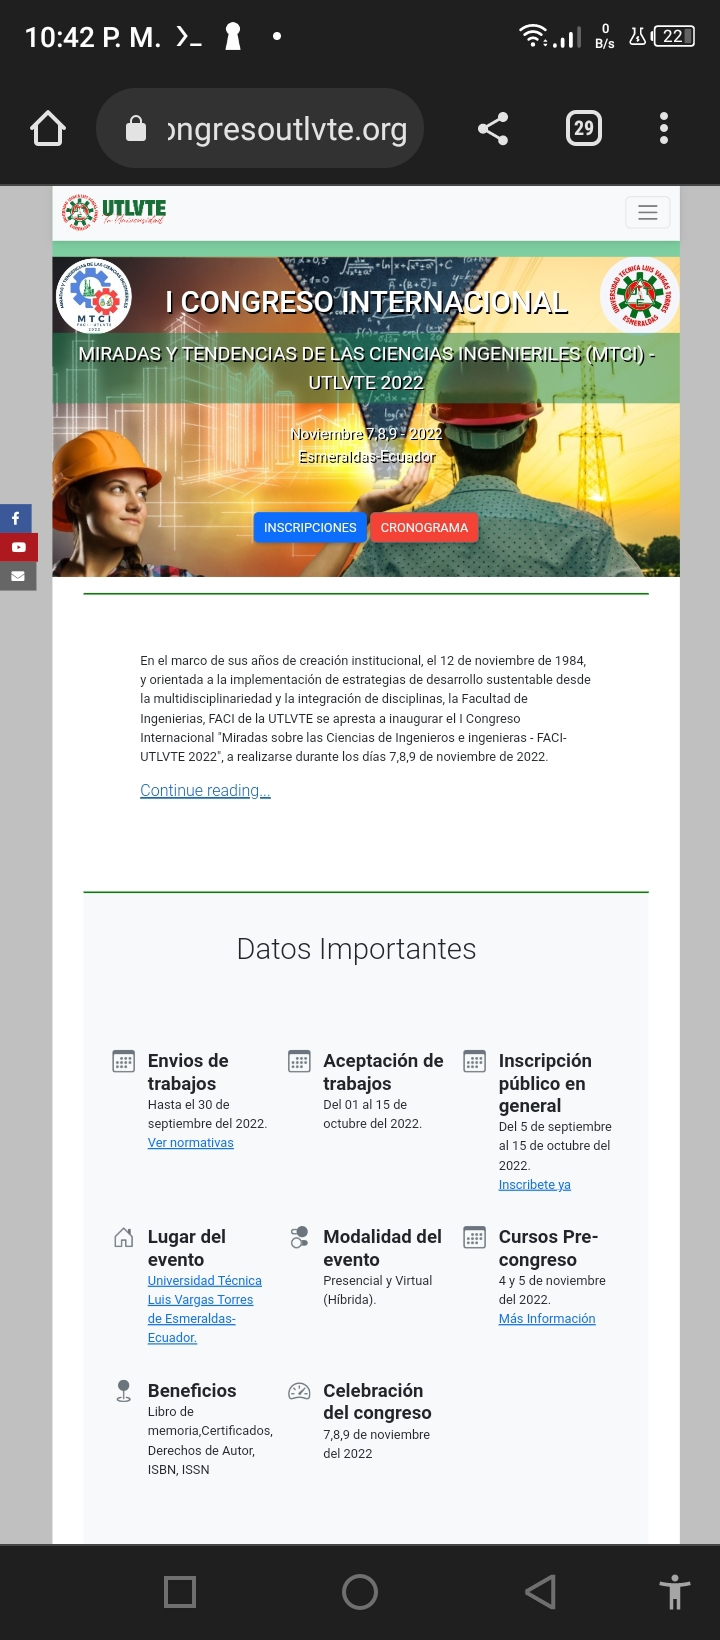
\includegraphics[scale=0.3]{index1.jpg}
  \caption{index1.php }
  \label{fig:arquitectura1}
\end{figure}
  
\end{minipage}
\hspace{0.5cm}
        \begin{minipage}[H]{0.45\linewidth}
\begin{figure}[H]
  \centering
  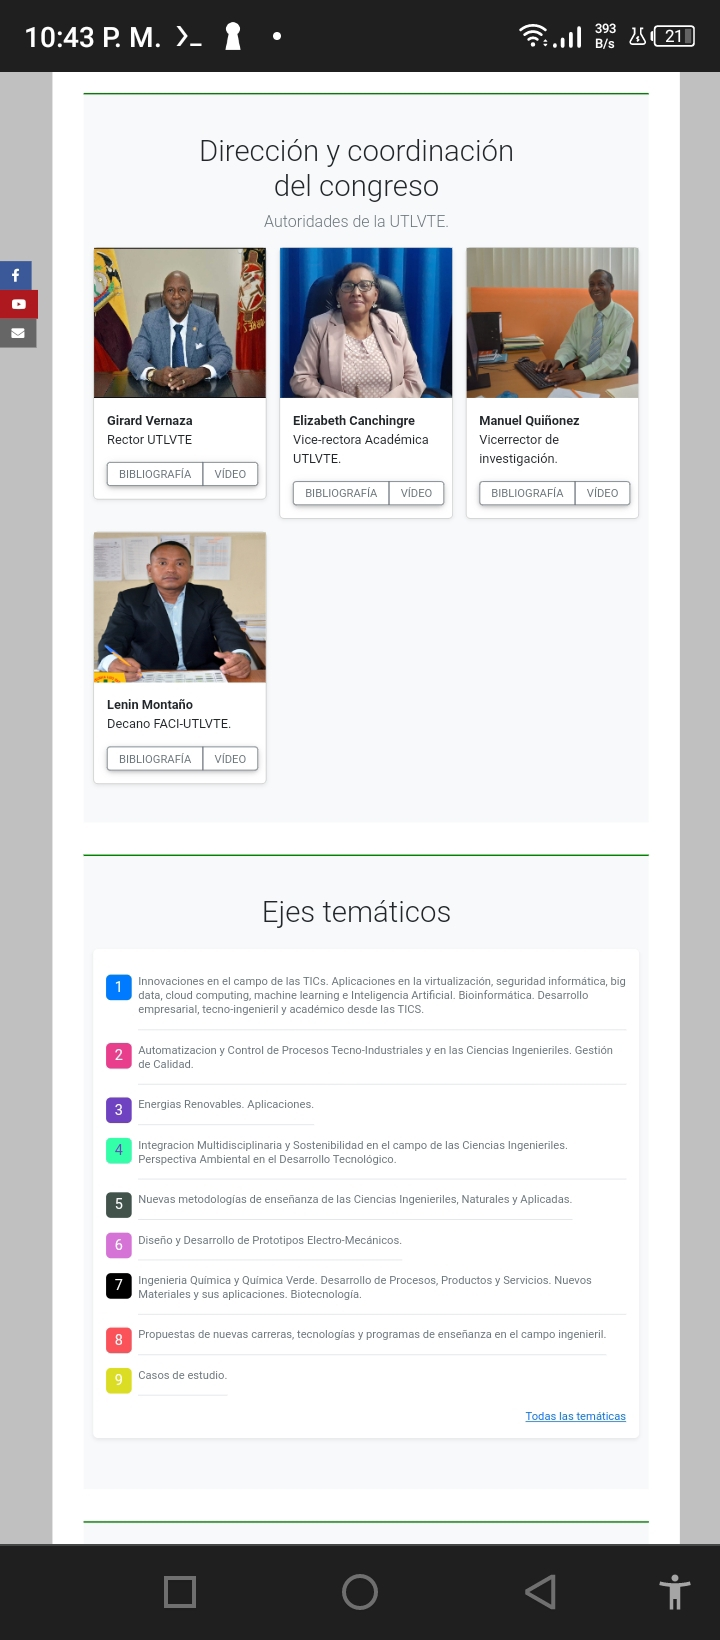
\includegraphics[scale=0.3]{index2.jpg}
  \caption{index2.php }
  \label{fig:arquitectura2}
\end{figure}
  
\end{minipage}





\begin{minipage}[H]{0.45\linewidth}
\begin{figure}[H]
  \centering
  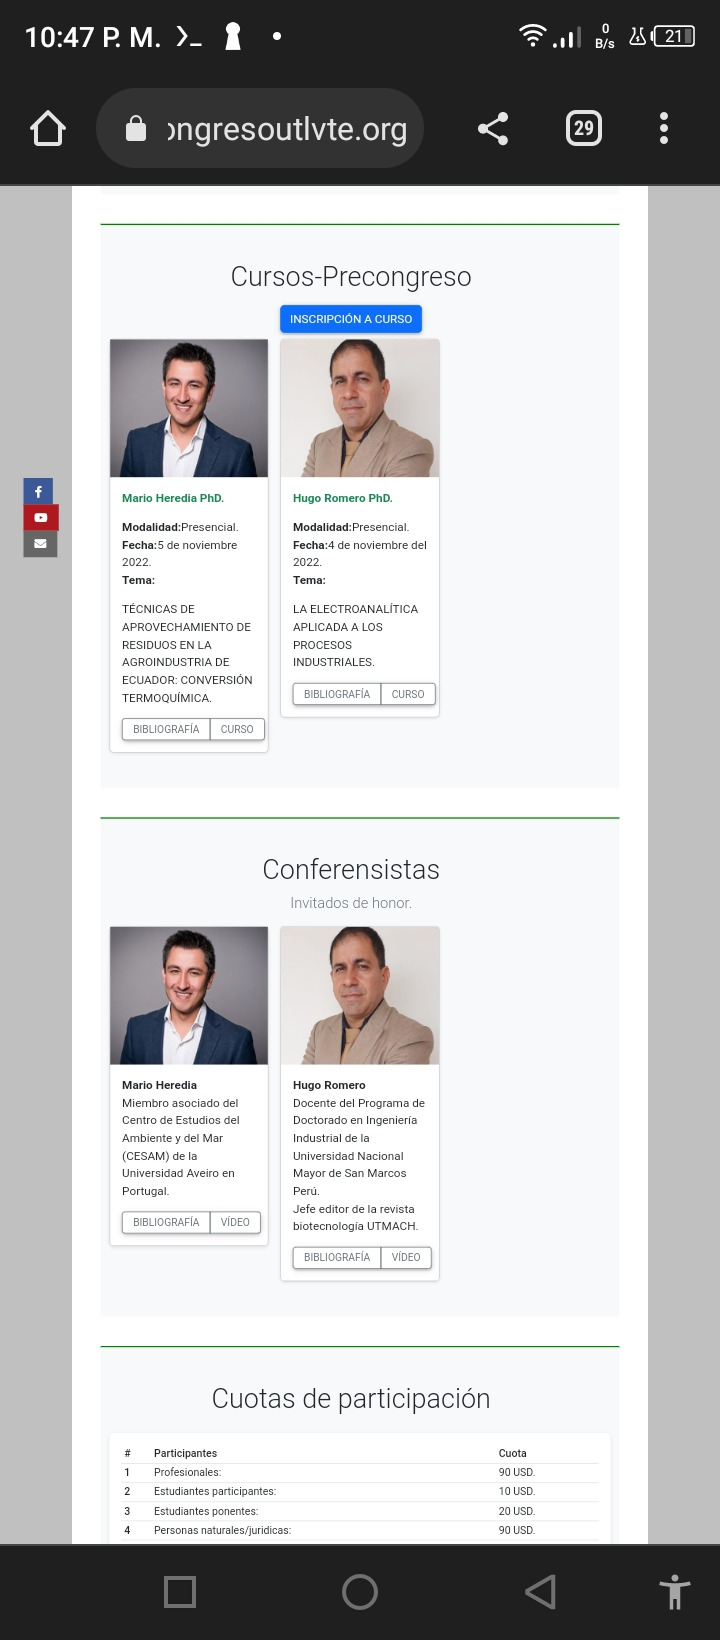
\includegraphics[scale=0.3]{index3.jpg}
  \caption{Se muestra conferencistas en primera página }
  \label{fig:arquitectura1}
\end{figure}
  
\end{minipage}
\hspace{0.5cm}
        \begin{minipage}[H]{0.45\linewidth}
\begin{figure}[H]
  \centering
  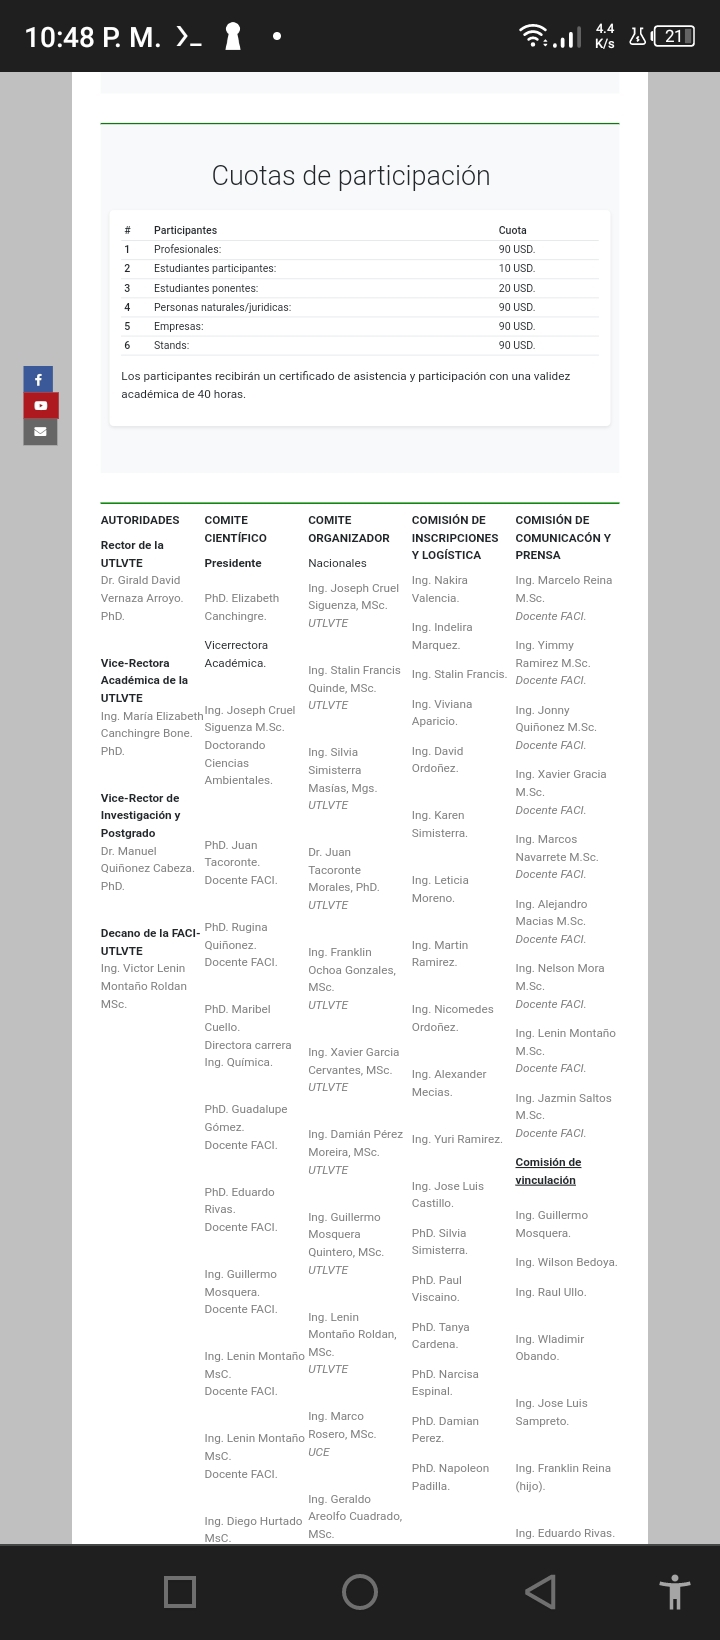
\includegraphics[scale=0.3]{index4.jpg}
  \caption{Se muestra los comites y sus miembros }
  \label{fig:arquitectura2}
\end{figure}
  
\end{minipage}













\newpage
\subsection{Página de presentación del congreso }
\label{sec:pagina-principal}

En la figura \ref{fig:presentacion}, se muestra el motivo, la visión, la misión y los  objetivos del congreso, información que forma parte de la presentación del evento.


\begin{figure}[H]
  \centering
  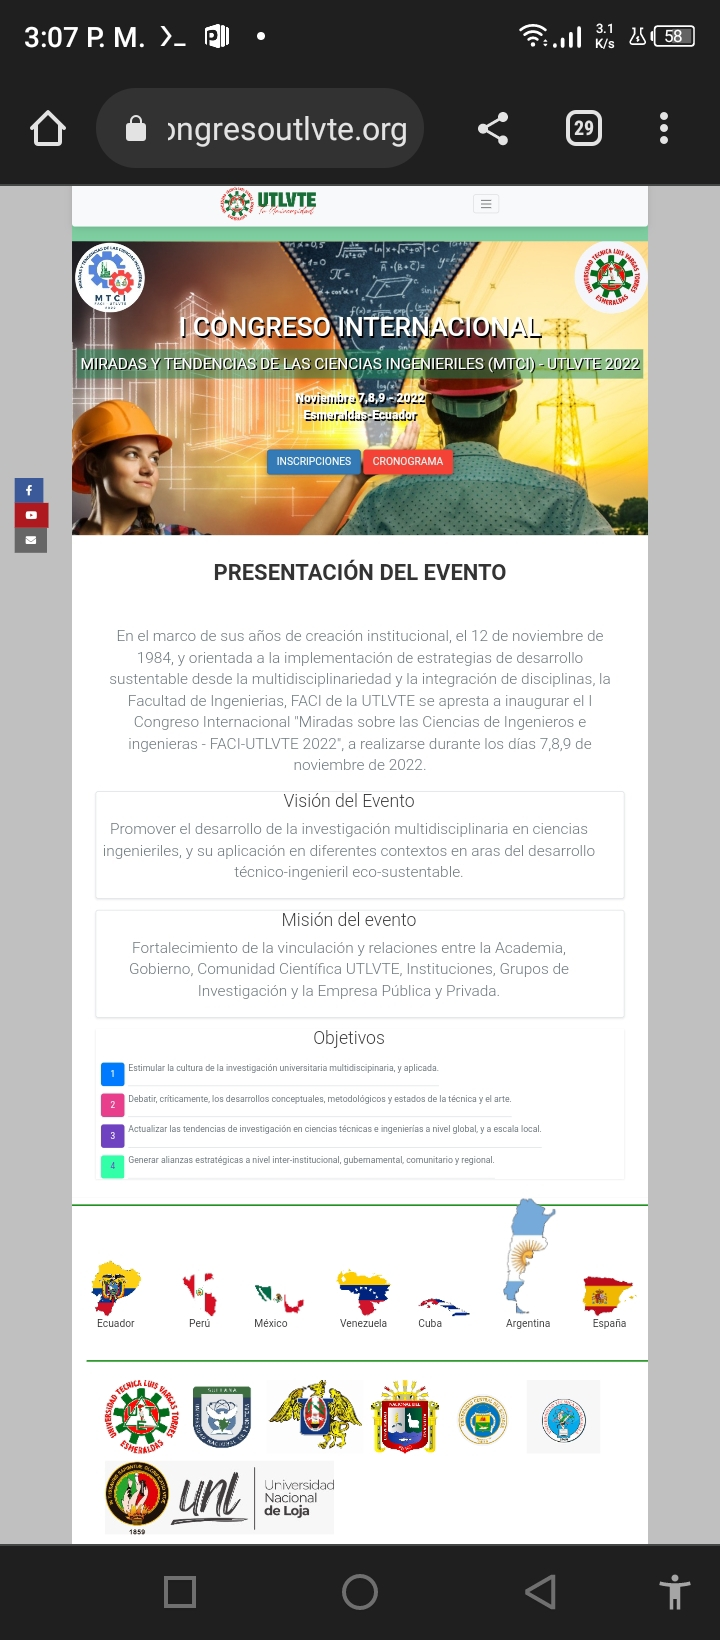
\includegraphics[scale=0.3]{presentacion.jpg}
  \caption{Presentación del congreso}
  \label{fig:presentacion}
\end{figure}

\newpage
\subsection{Página de normas de presentación }
\label{sec:pagina-principal}

Esta es la página  donde se muestra las normas a seguir para que los ponentes entreguen sus trabajos de forma correcta.


\begin{minipage}[H]{0.45\linewidth}
  \begin{figure}[H]
    \centering
    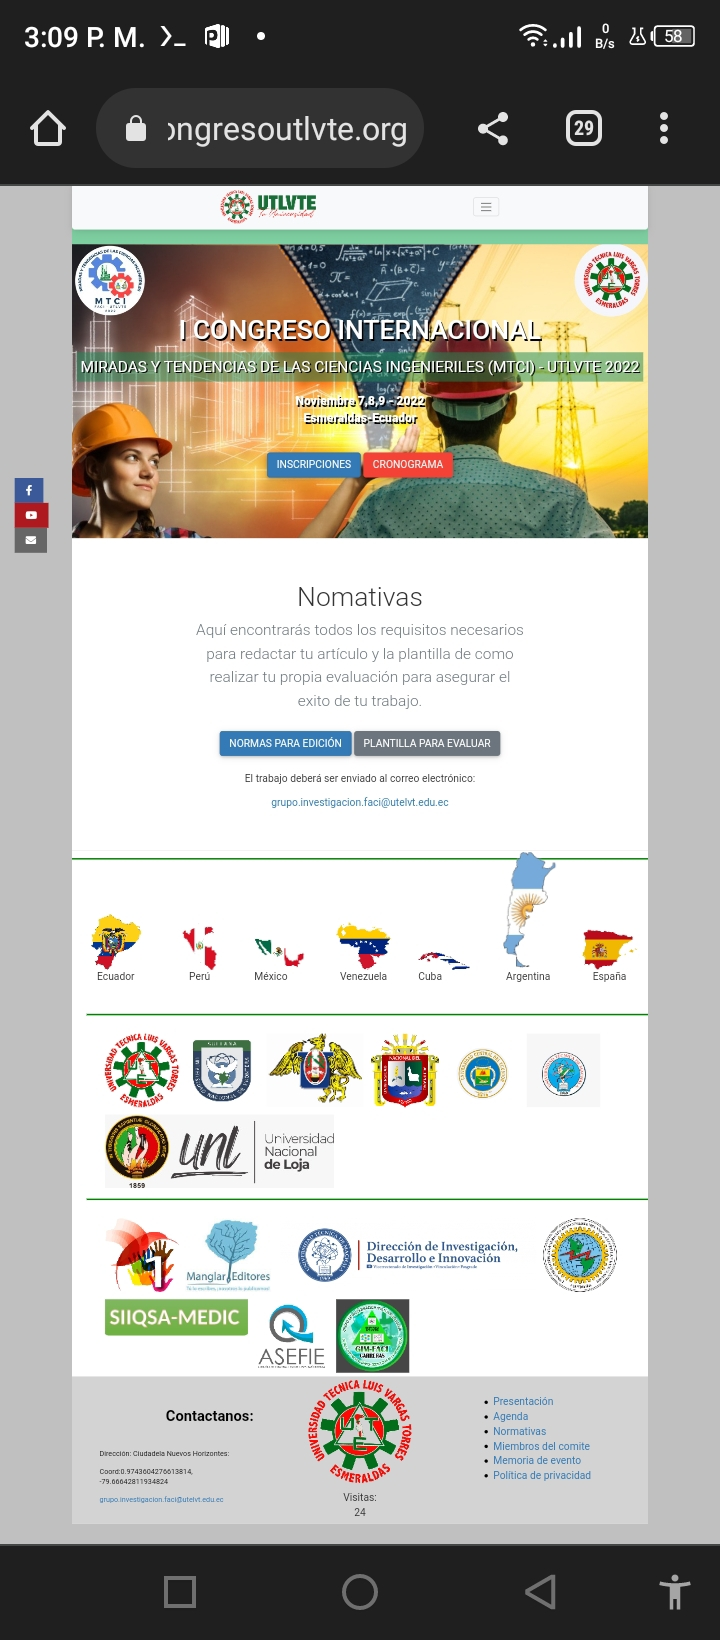
\includegraphics[scale=0.3]{normativas.jpg}
    \caption{Normativas}
    \label{fig:arquitectura}
  \end{figure}

\end{minipage}




\newpage
\subsection{Página de temáticas }
\label{sec:pagina-principal}

La conferencias preparadas por los ponentes debe realizarse en función de ejes temáticos definidos por la unidad de investigación de la Universidad auspiciante.

\begin{minipage}[H]{0.5\linewidth}
  \begin{figure}[H]
    \centering
    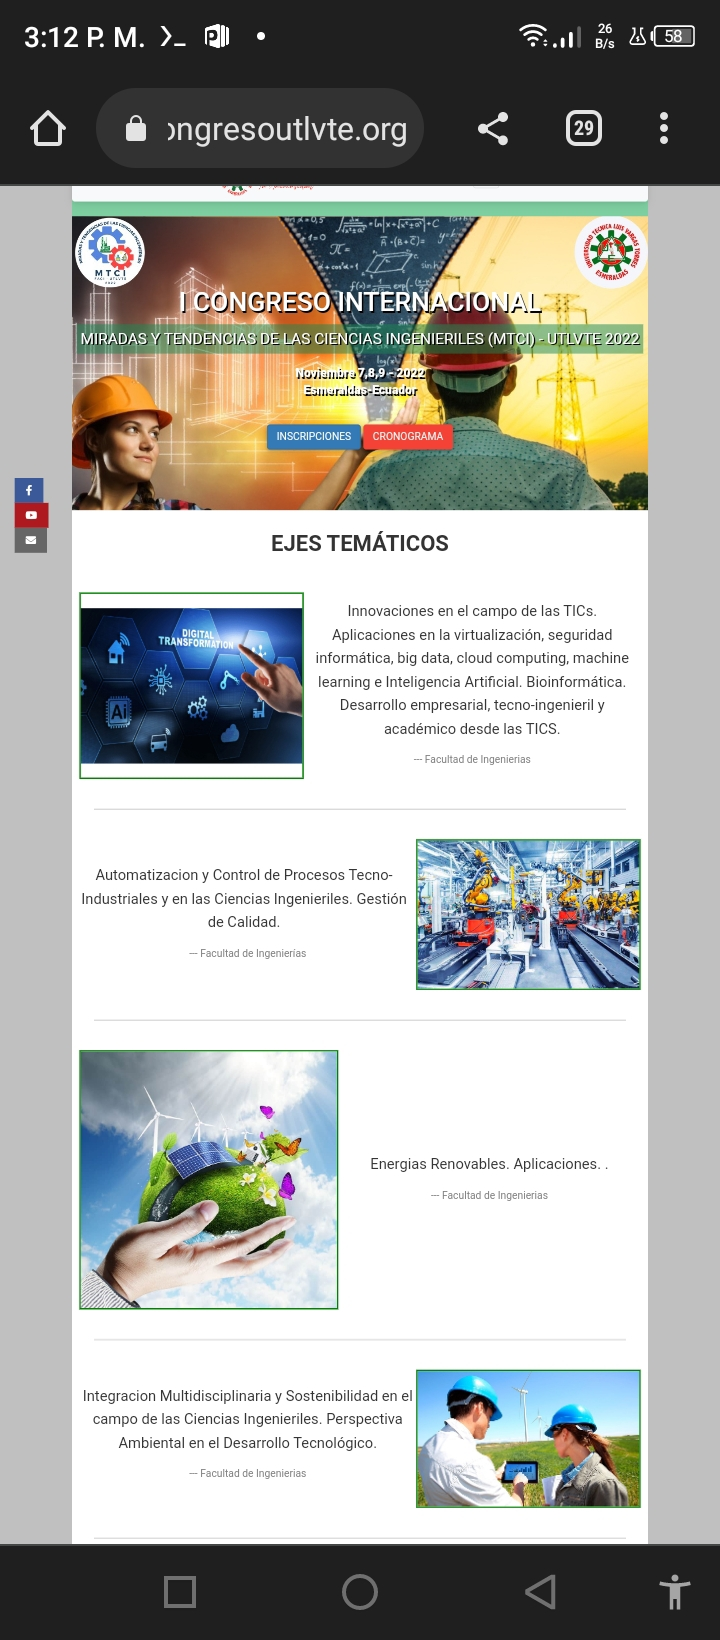
\includegraphics[scale=0.3]{tematicas.jpg}
    \caption{Temáticas}
    \label{fig:tematicas1}
  \end{figure}
\end{minipage}
\hspace{0.5cm}
\begin{minipage}[H]{0.5\linewidth}
  \begin{figure}[H]
    \centering
    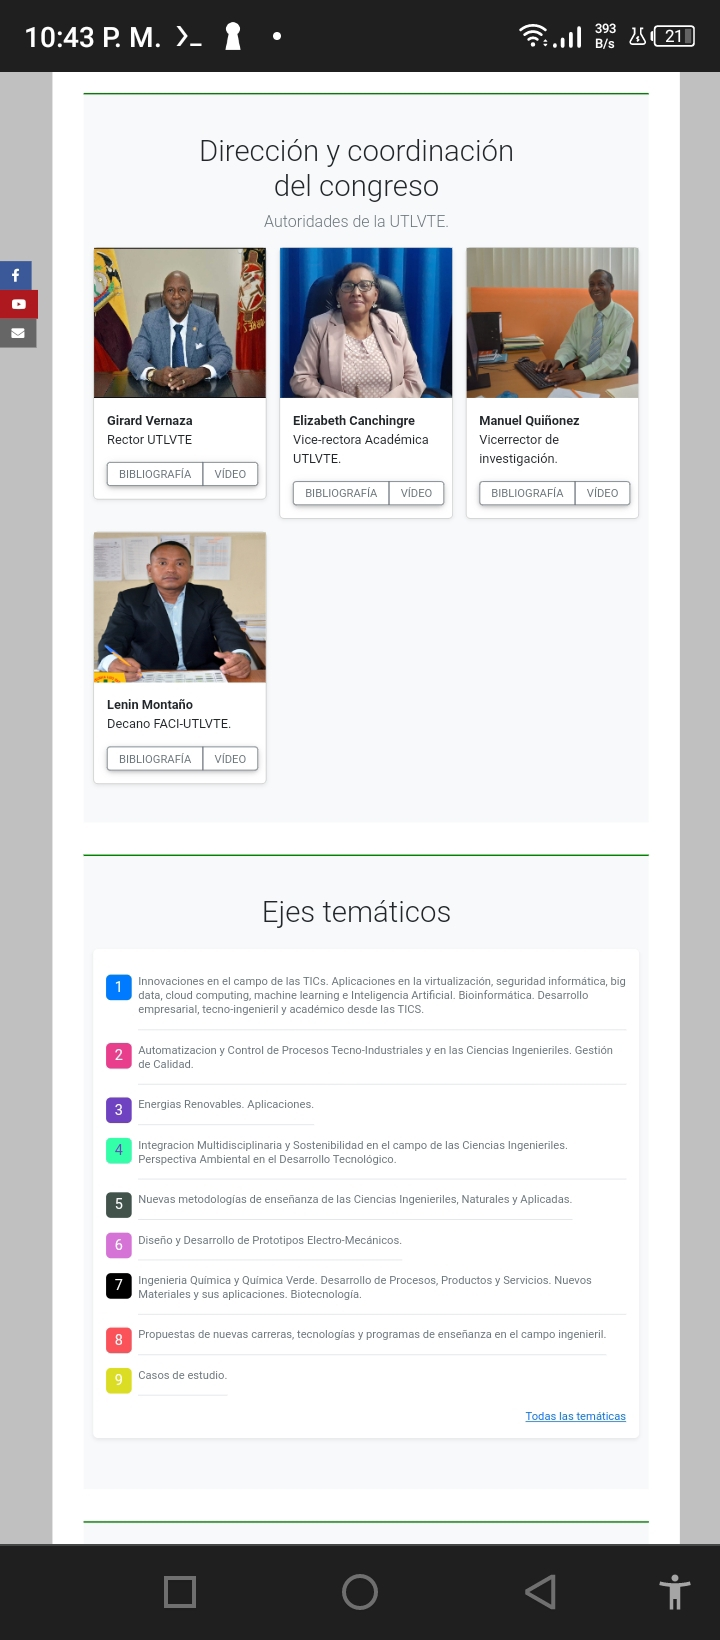
\includegraphics[scale=0.3]{index2.jpg}
    \caption{Temáticas en página principal}
    \label{fig:tematicas2}
  \end{figure}
\end{minipage}

\newpage
\subsection{Página de confencistas }
\label{sec:pagina-principal}

Los temas y los conferencistas son mostrados en esta página, los usuarios también tendrán acceso a una hoja de vida resumida para conocer detalles sobre el conferencista.

  

\begin{minipage}[H]{0.5\linewidth}
  \begin{figure}[H]
    \centering
    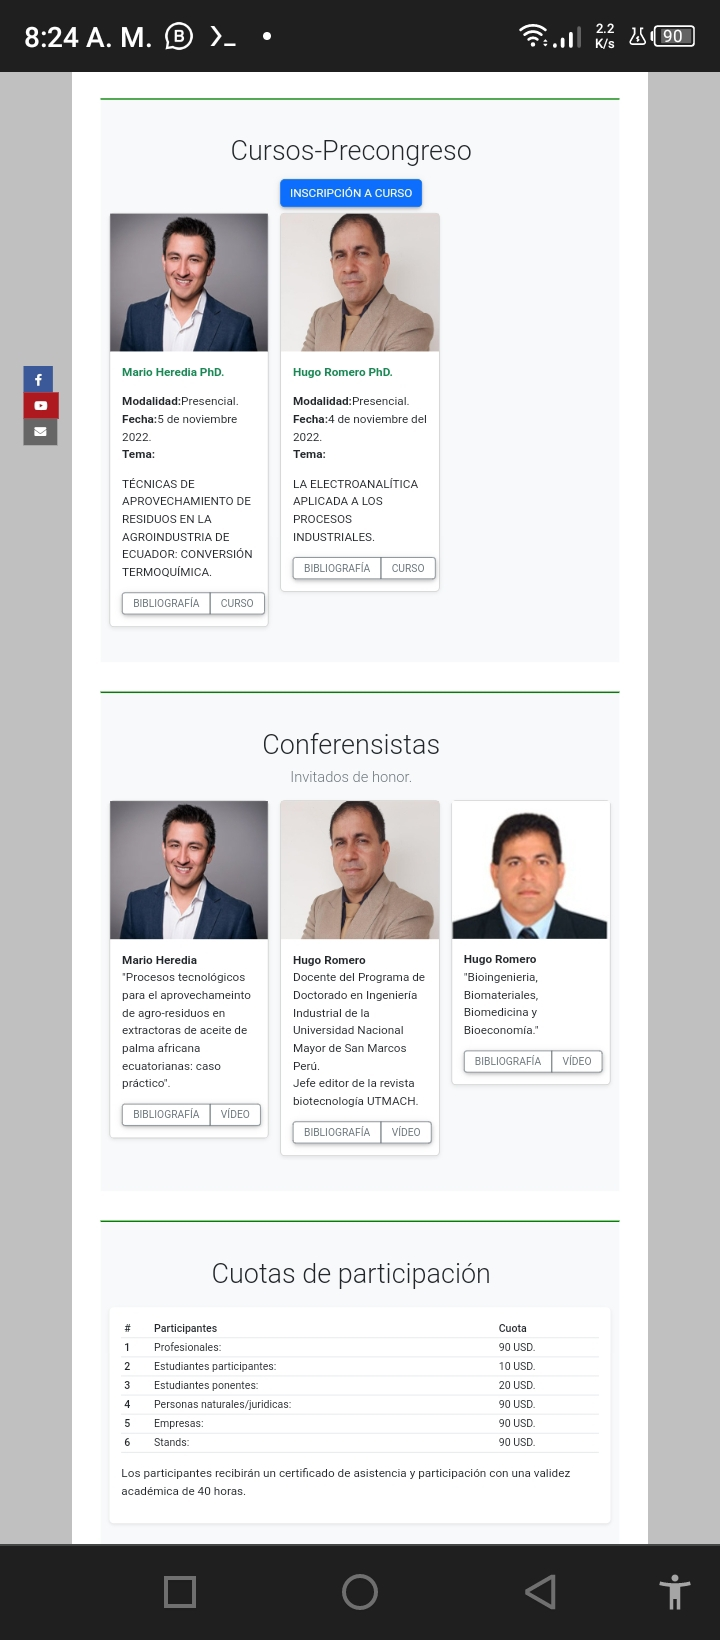
\includegraphics[scale=0.3]{conferencistas.jpg}
    \caption{Lista de conferensistas}
    \label{fig:conferensistas}
  \end{figure}
\end{minipage}
\hspace{0.5cm}
\begin{minipage}[H]{0.5\linewidth}
  \begin{figure}[H]
    \centering
    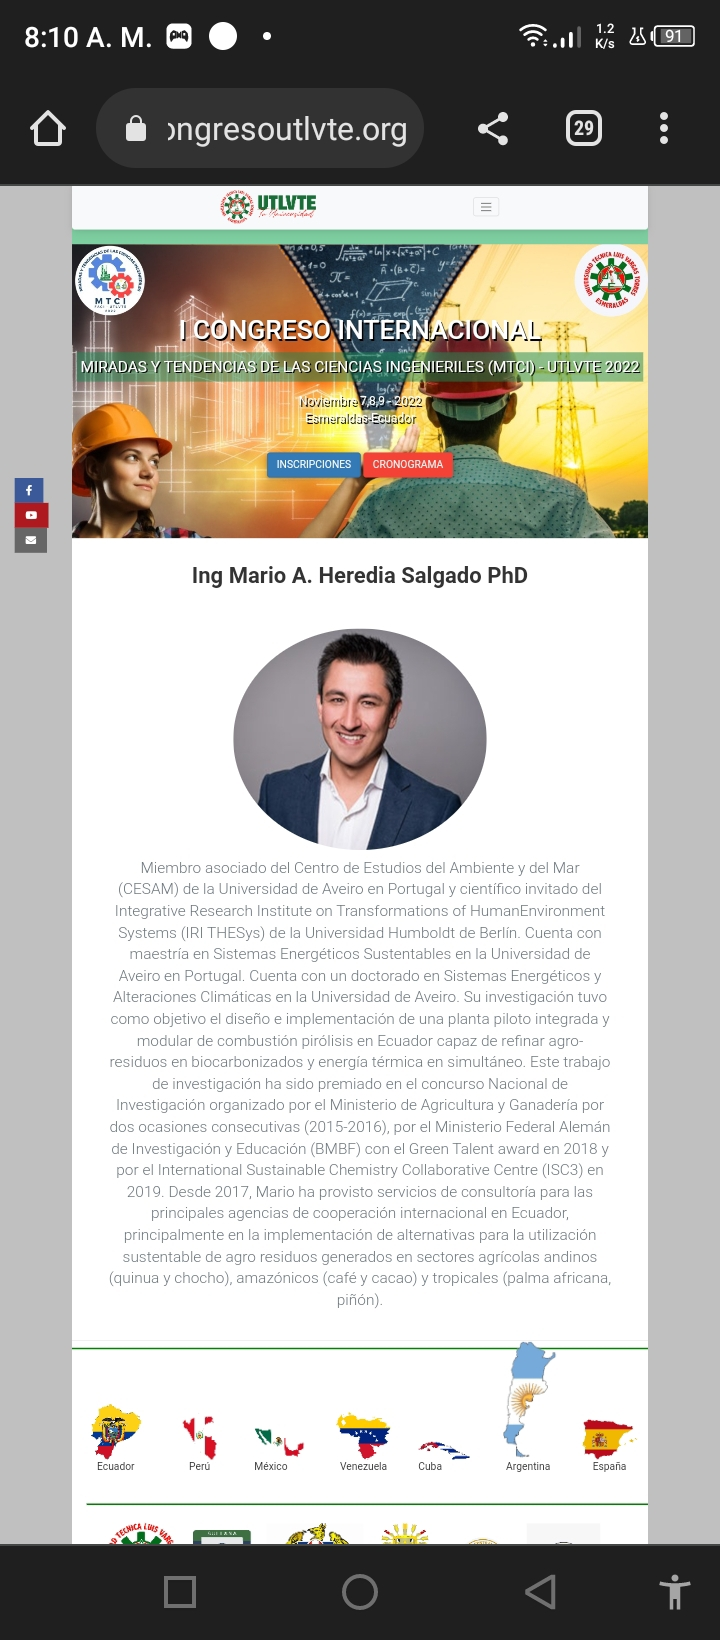
\includegraphics[scale=0.3]{bibliografia.jpg}
    \caption{Bibliografía del conferensista}
    \label{fig:bibliografia}
  \end{figure}
\end{minipage}



  





\newpage
\subsection{Página para mostrar la memoria generada}
\label{sec:pagina-principal}

En esta página web se presenta todo los afíches generados y difundidos para dar a conocer el evento del congreso a realizarse..


\begin{figure}[H]
  \centering
  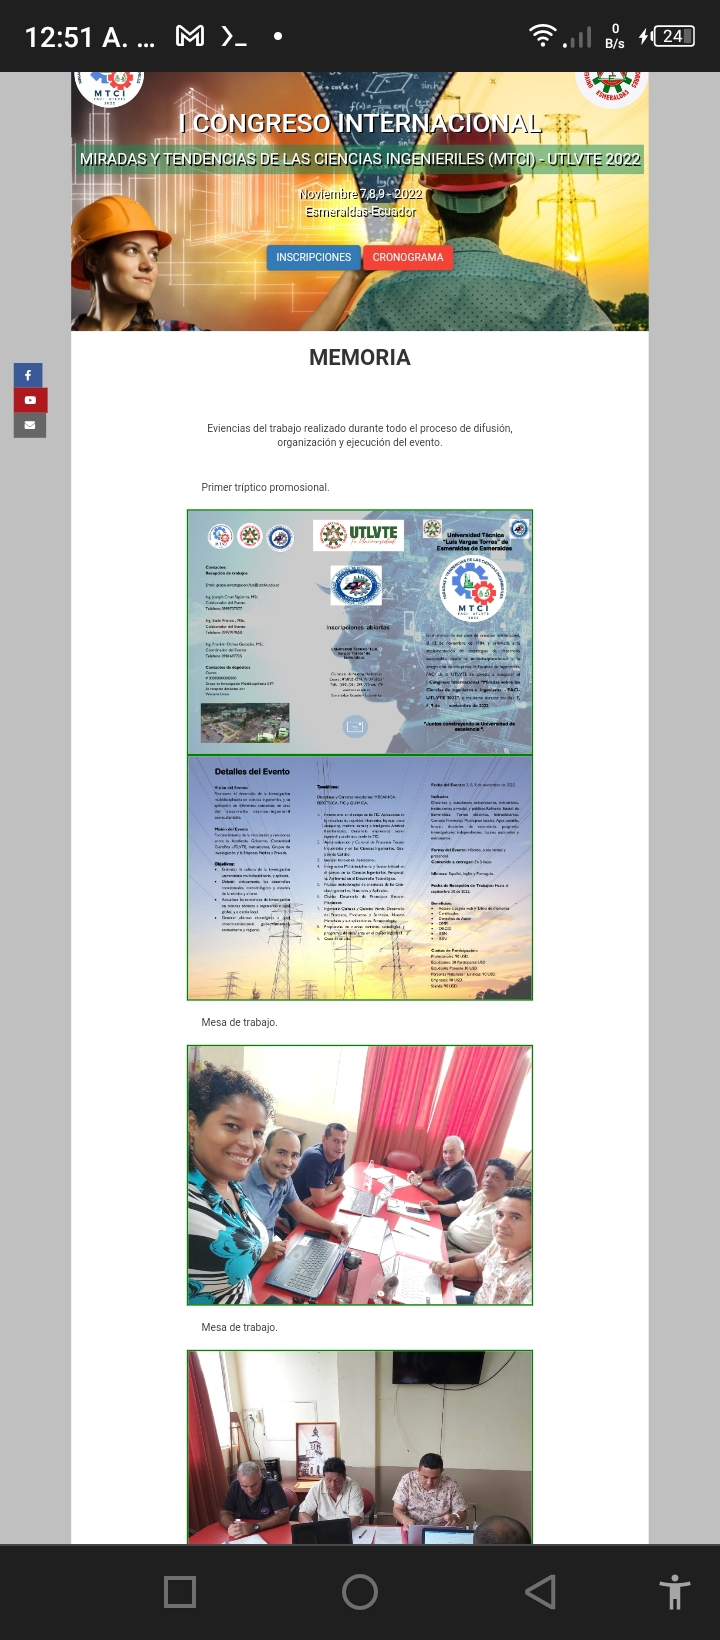
\includegraphics[scale=0.3]{memoria.jpg}
  \caption{Memoria}
  \label{fig:arquitectura}
\end{figure}

\newpage
\subsection{Página para inscripciones }
\label{sec:pagina-principal}

Esta página web permite acceder a un registro o formulario donde las personas que quieren participar en el congreso puedan dejar sus datos personales, datos que serán utilizados para generar los certificados respectivos.


\begin{minipage}[H]{0.45\linewidth}
  \begin{figure}[H]
    \centering
    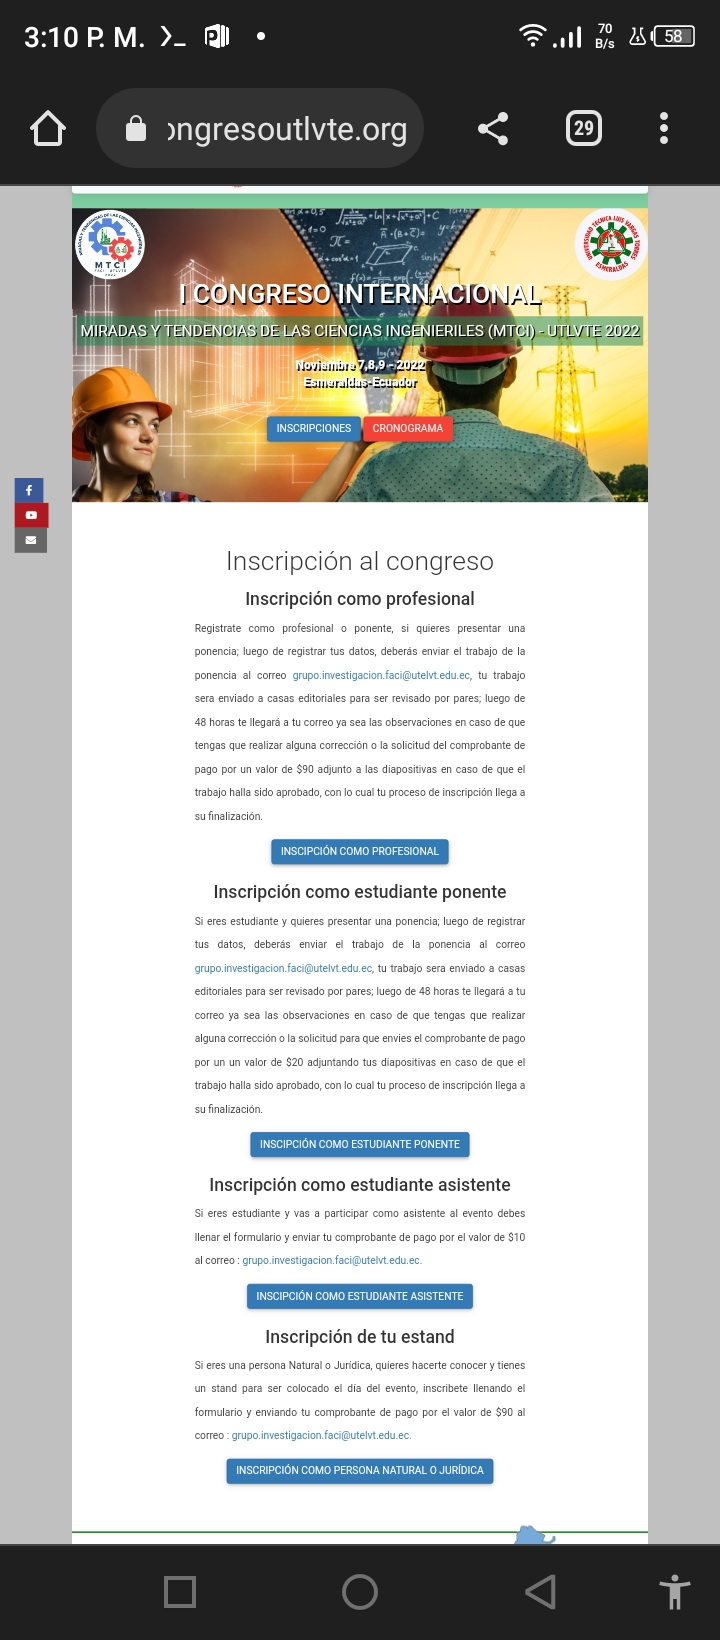
\includegraphics[scale=0.3]{inscripcion.jpg}
    \caption{Inscripciones al congreso}
    \label{fig:arquitectura}
  \end{figure}
\end{minipage}
\begin{minipage}[H]{0.45\linewidth}
  \begin{figure}[H]
    \centering
    
\includegraphics[scale=0.3]{inscripcion2.jpg}
    \caption{Formulario de inscripción}
    \label{fig:arquitectura2}
  \end{figure}
\end{minipage}




\end{document}

%%% Local Variables:
%%% mode: latex
%%% TeX-master: t
%%% End:
